\chapter{Content chapter}

Unless the chapter heading already makes it clear, an introductory paragraph that explains how this chapter contributes to the objectives of the report/project.

\section{Heading level 2}

\subsection{Heading level 3}

\subsubsection{Deepest heading, only if you cannot do without it}
\vspace{2cm}

\paragraph{Equations:}

An equation must read like part of the text. The solution of the quadratic equation $ax^2+bx+c=0$ given by the following expression (note the full stop after the equation to indicate the end of the sentence):
\begin{equation}
    x = \frac{-b \pm \sqrt{b^2-4ac}}{2b} .
\end{equation}
In other cases the equation is in the middle of the sentence. Then the paragraph following the equation should start with a small letter. Euler's identity is 
\begin{equation}
    e^{i \pi} + 1 = 0 ,
\end{equation}
where $e$ is Euler's number, the base of natural logarithms.

The \texttt{amsmath} has a wealth of structure and information on formatting of mathematical equations.

\pagebreak
\paragraph{Symbols and numbers:}

Symbols that represent values of properties should be printed in italics, but SI units and names of functions (e.g. sin, cos and tan) must not be printed in italics. There must be a small hard space between a number and its unit, e.g. \qty{120}{km}. Use the \texttt{siunitx} package to typeset numbers, angles and quantities with units:
\begin{tabbing}
\hspace*{\parindent}\=\verb|\qty{20}{N.m}|\quad\=$\rightarrow$\quad\=\kill
    \>\verb|\num{1.23e3}| \>$\rightarrow$\> \num{1.23e3} \\
    \>\verb|\ang{30}|     \>$\rightarrow$\> \ang{30} \\
    \>\verb|\qty{20}{N.m}|\>$\rightarrow$\> \qty{20}{N.m}
\end{tabbing}

\paragraph{Figures and tables:}
The \texttt{graphicx} package can import \texttt{PDF}, \texttt{PNG} and \texttt{JPG} graphic files.

\begin{table}[htbp]
    \centering
    \caption{Standard ISO paper sizes}
    \label{tab:paper}
    \begin{tabular}{lcccc}
    \hline
        Paper\quad && \multicolumn{3}{c}{Sizes} \\
    \cline{2-5}
        &&  $W$      && $H$ \\
        && \small [mm] &&  \small [mm]   \\
    \cline{1-1}\cline{3-3}\cline{5-5}
        A0 && 841 && 1189 \\
        A1 && 594 &&  841 \\
        A2 && 420 &&  594 \\
        A3 && 297 &&  420 \\
        A4 && 210 &&  297 \\
        A5 && 148 &&  210 \\
    \hline
    \end{tabular}
\end{table}


\begin{figure}[htbp]
    \centering
    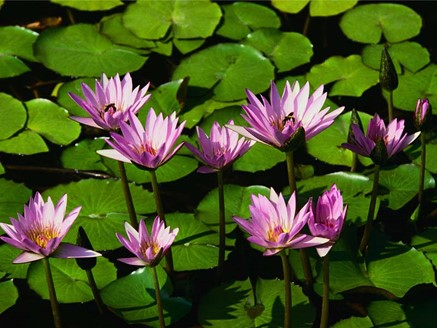
\includegraphics[scale=0.75]{figs/waterplants}
    \caption{Water plants}
    \label{fig:waterplant}
\end{figure}
